\documentclass[11pt, a4paper]{article}
\usepackage{amsmath,amsthm, graphicx}
\usepackage{verbatim}
\title{ELEN4009 - Software Engineering\\Smart Home Power Management System\\Software Requirement Specification}
\author{Ari Croock (718005)\\Kanaka Babshet (678851)\\Alice Yang (597609)\\Daniel Weinberg (547937)}
\date{\today}

\begin{document}
	\maketitle
	\section{Introduction}
	\subsection{Purpose}
	This document details the system requirements specification for the Smart Home Power Management System. The system design document will be developed from this document.\\
	
	With the rapidly growing interest in new Internet of Things (IoT) technologies, networks consisting of these devices will become increasingly difficult to manage and control. Additionally, power consumption and monitoring will become a greater concern, especially in emerging markets such as South Africa.\\
	
	This project aims to provide a flexible software system which is able to remotely control and monitor IoT devices, as well as perform detailed power consumption diagnostics.
	
	\subsection{Project Scope}
	The project is a system that will allow for remote control, monitoring and automation of IoT devices on a Local Area Network (LAN). A client-server architecture will be used since this allows a back-end server to continuously manage devices while allowing for a client to connect on-demand. The front-end will initially be implemented as a web page for simplicity and compatibility with many existing devices (such as cellphones and personal computers).
	
	The back-end provides functionality to control and monitor devices, and to log device power consumption. Additionally, the back-end will contain the web server used for interfacing with users.
	
	The front-end will consist of a web-based user interface which will allow secure access to a device dashboard. The dashboard will provide remote control and configuration of devices, as well as access to power consumption data. Addition and removal of IoT devices will also be performed through the dashboard. 
	
	\section{Project Overview}
	\begin{figure}
		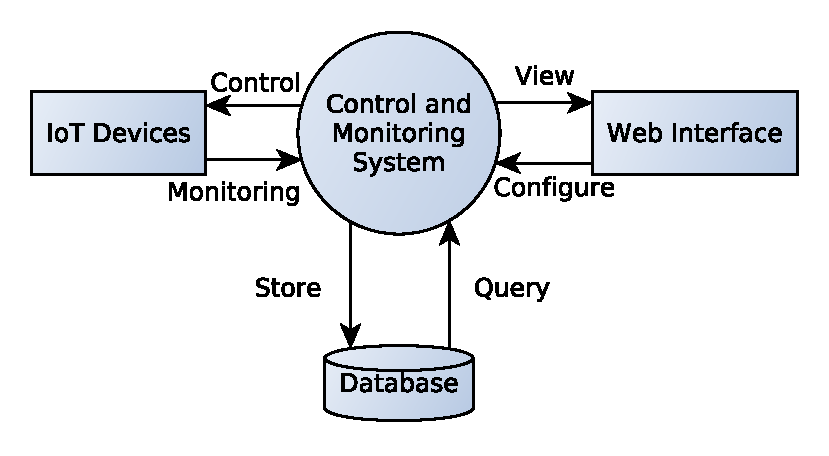
\includegraphics[width=\columnwidth]{data-flow-1}
		\caption{Data flow diagram (DFD) of the system. All data flows are bidirectional}
	\end{figure}
	
	%3 tier has better security because 2 tier the client is allowed access and communication with 
	
	\section{External Interface Requirements}
	The external interface is the interface which allows the user to interact with the system through a hardware device using software. The external interfaces consists of a user interface, hardware interface, software interface and communication interface. 
	
	\subsection{User Interface - GUI}
	The user interface is how the user will interact with the system. The requirements for the design of user interface must be simple and easy to navigate. A simple format of representing all the devices connected to the Smart Home Power Management System is to display the features available for all devices on a dashboard. This can been seen in Figure \ref{Home_Dashboard}.
	
	\begin{itemize}
		\item Home Page Dashboard
			\begin{figure}[h!]
				\centering
				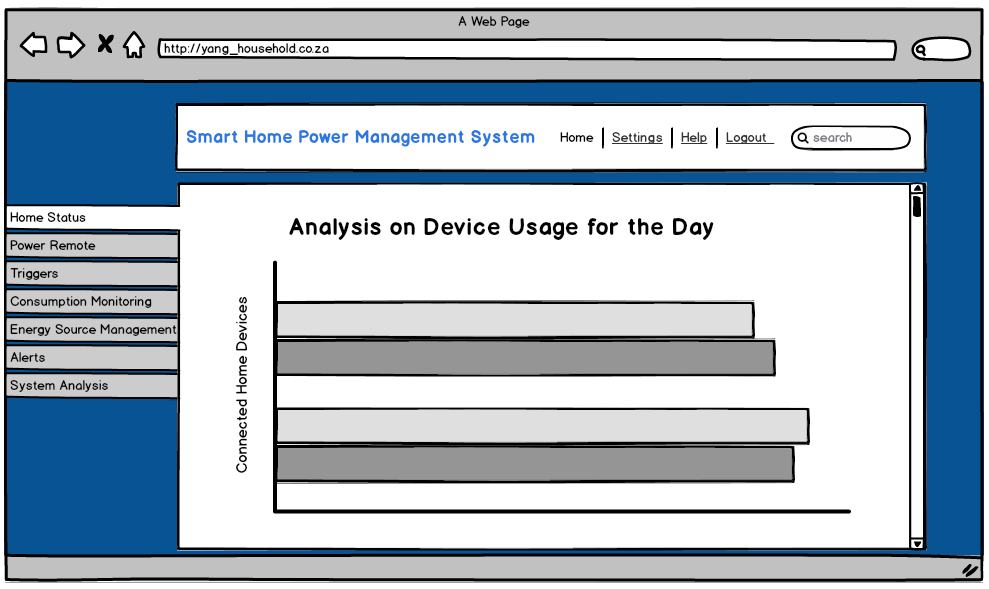
\includegraphics[scale=0.5]{Home_Page.png}
				\caption{Figure illustrating the home page the user will see once they have logged on to access the system.}
				\label{Home_Dashboard}
			\end{figure}
		\item Trigger Tab on Dashboard
			\begin{figure}[h!]
				\centering
				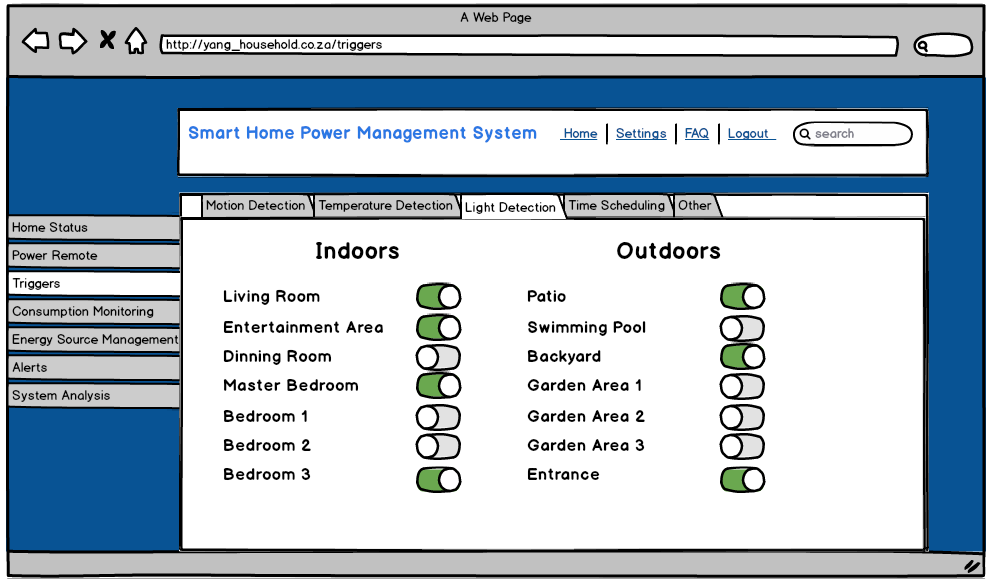
\includegraphics[scale=0.5]{Trigger_Tab.png}
				\caption{Figure illustrating the triggers tab, to allow users to control switching of sensors in their home through the system.}
				\label{Trigger_Tab}
			\end{figure}
		\pagebreak
		\item Settings Page
			\begin{figure}[h!]
				\centering
				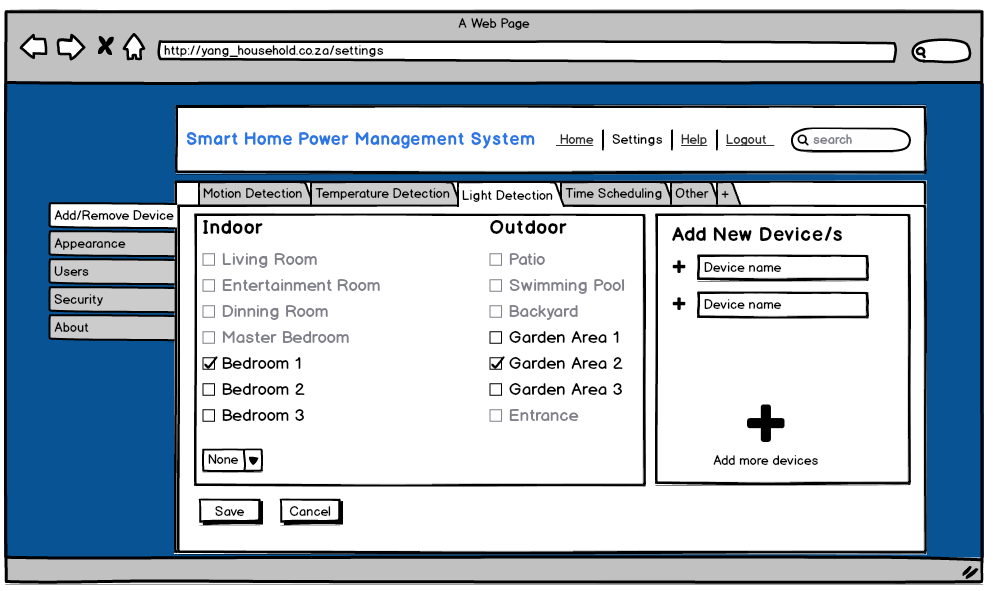
\includegraphics[scale=0.5]{Settings.png}
				\caption{Figure illustrating the settings page.}
				\label{Settings}
			\end{figure}
	\end{itemize}
	
	
	\pagebreak
	\subsection{Hardware Interface}
	The user interface is implemented on a web based platform that is accessible through a browser. The hardware required to access the system can be either of the listed devices found in the list below:
	
	\begin{enumerate}
		\item Large Desktops (1200 -  pixels)
		\item Medium Desktops (992 - 1199 pixels)
		\item Small Devices (768 - 991 pixels)
		\item Extra Small Devices (max 767 pixels)
	\end{enumerate}
	
	
	
	
	\section{Other Non-Functional Requirements}
	
	\subsection{Performance Requirements}
	The smart home power system is an application and system that is designed for efficiency. This means that the application as well as the connecting household components need to respond quickly and in real time. 
	\\\\
	The application will most likely undergo several updates and changes for the user's benefit. The system is required to update on user command. Updates will include further improvements to the application as well as fixes for issues that arise in operation.
	
	\subsection{Safety Requirements} 
	The application as well as the system components need to take certain safety concerns into account. 
	\\\\
	Due to the fact that the application is essentially controlling most of a home's appliances and electricity usage, it is important that it monitors everything it is controlling to prevent problems that may arise. The application needs to ensure that any device connected in the system does not reach a dangerous level of usage. In this case, the application should either switch off the device in question or notify the user that something is not functioning correctly and needs to be addressed. 
	
	\subsection{Security Requirements}
	Due to the fact that the system controls a user's home, it therefore requires security considerations to be taken into account.
	\\\\
	The system needs to ensure that only the user has access to the application to prevent external parties gaining control of the connected components within a house. This can be done with a signup, login and authentication process. 
	The components within the house that the application connects with, need to be protected from external parties and therefore they must be explicitly authenticated. 
	
	\subsection{Software Quality Attributes}
	The application is web based and needs to be user friendly. The functioning of the application needs to be simple so that no additional documentation or prior knowledge or experience is required. 
	
	
\end{document}